\documentclass[12pt, a4paper]{article}
\usepackage[utf8]{inputenc}
\usepackage[T1]{fontenc}
\usepackage[textwidth = 460pt,top = 80pt, bottom = 80pt]{geometry}
\usepackage{graphicx}
\usepackage[justification=default]{subfig} 
\usepackage[update]{epstopdf}
\usepackage[labelfont=bf]{caption}
\usepackage[dvipsnames]{xcolor}
\usepackage{fancyhdr}
\usepackage{booktabs}
\usepackage{multicol}
\usepackage{multirow}
\usepackage{titling}
\usepackage{float}
\usepackage{bm}
\usepackage[intlimits]{empheq}
\usepackage[hidelinks]{hyperref}
\usepackage{amsmath}
\usepackage{graphicx}
\usepackage{subcaption}
\usepackage{amssymb}

\usepackage{tikz}
\usepackage{listings}
\lstset{
    basicstyle=\small\ttfamily,
    keywordstyle=\color{blue}\bfseries,
    commentstyle=\color{gray}\itshape,
    stringstyle=\color{red},
    numbers=none,
    breaklines=true,
    showstringspaces=false,
    tabsize=4
}
\usetikzlibrary{positioning,3d,shapes.geometric, arrows.meta, fit}


%Bibliography

\usepackage{csquotes}
\usepackage[sorting=none,%
sortcites=true,%
bibencoding=ascii,%
autopunct=true,%
hyperref=true,%
language=auto,%
%backref=true,%
url=false,%
%maxcitenames=10,%
%minbibnames = 20,%
maxbibnames = 3,%
giveninits, 
natbib = false,
isbn=false,%
backend=biber]{biblatex}
\addbibresource{references.bib}

\usepackage[]{hyperref}
\usepackage{cleveref}
%%% CREF setup
\crefname{equation}{Eq.}{Eqs.}
\crefname{table}{Table}{Tables}
\crefname{figure}{Fig.}{Figs.}


\begin{document}

\begin{titlingpage}
    \begin{center}
        \begin{figure}
            \centering
            \includegraphics[width=0.6\textwidth]{figures/logopolimi_mod.jpg}
        \end{figure}
        \Large{\textsc{Politecnico di Milano \\ School of Industrial and Information Engineering \\ M.Sc. in High Performance Computing}}

        \vspace{1cm}

        \rule{0.95\textwidth}{0.7mm}
        {\Large{\textbf{Hybrid thread-MPI parallelization for ADR equation}}}
        \rule{0.95\textwidth}{0.7mm}

        \vspace{1cm}

        \large{\textbf{Peng Rao}, \textbf{Jiali Claudio Huang}, \textbf{Ruiying Jiao}}

        \vspace{1cm}

        \small{\textbf{Repo: \href{https://github.com/Peng-Rao/HybridADRSolver}{https://github.com/Peng-Rao/HybridADRSolver}}}
    \end{center}

\end{titlingpage}

\pagenumbering{roman}

\tableofcontents

\clearpage

\setcounter{page}{1}
\pagenumbering{arabic}

\section{Problem statement} \label{sec:problem_statement}
\subsection{Strong formulation}
Consider the following \textbf{Advection-Diffusion-Reaction} equation with mixed Dirichlet-Neumann boundary conditions:
\[
    \begin{cases}
        -\nabla \cdot (\mu \nabla u) + \nabla \cdot (\boldsymbol{\beta} u) + \gamma u = f
         & \text{in } \Omega,                                         \\[0.5em]
        u = g
         & \text{on } \Gamma_D \subset \partial \Omega,               \\[0.5em]
        \nabla u \cdot \boldsymbol{n} = h
         & \text{on } \Gamma_N = \partial \Omega \setminus \Gamma_D .
    \end{cases}
\]
where:
\begin{itemize}
    \item $\Omega \subset \mathbb{R}^d$ (with $d = 1, 2, 3$) is an open bounded domain with boundary $\partial \Omega$;
    \item $\mu > 0$ is the diffusion coefficient;
    \item $\boldsymbol{\beta} \in [L^{\infty}(\Omega)]^d$ is the advection velocity field;
    \item $\gamma \geq 0$ is the reaction coefficient;
    \item $f \in L^2(\Omega)$ is a source term;
    \item $g \in H^{1/2}(\Gamma_D)$ is the Dirichlet boundary data;
    \item $h \in L^2(\Gamma_N)$ is the Neumann boundary data;
    \item $\boldsymbol{n}$ is the outward unit normal vector on the boundary $\partial \Omega$.
    \item $u$ is the unknown scalar function to be solved for.
    \item $\Gamma_D$ and $\Gamma_N$ are the Dirichlet and Neumann parts of the boundary, respectively.
\end{itemize}

\subsection{Weak formulation}
We begin by defining the trial and test function spaces. To accommodate the non-homogeneous Dirichlet boundary condition, we introduce a \textit{lifting function} $u_g \in H^1(\Omega)$ such that $u_g = g$ on $\Gamma_D$:
\[
    V_g := \{ v \in H^1(\Omega) : v = g \quad \text{on } \Gamma_D \}
\]
The test space is the linear subspace of $H^1(\Omega)$ with homogeneous Dirichlet boundary conditions:
\[
    V_0 := \{ v \in H^1(\Omega) : v = 0 \quad \text{on } \Gamma_D \}
\]
Consequently, we decompose the solution as $u = u_0 + u_g$, where the unknown $u_0 \in V_0$.
\
Multiply the equation by a test function $v \in V_0$ and integrate over the domain $\Omega$:
\[
    \int_\Omega \left( -\nabla \cdot (\mu \nabla u) + \nabla \cdot (\boldsymbol{\beta} u) + \gamma u \right) v \, d\Omega = \int_\Omega f v \, d\Omega
\]
Using the linearity of the integral, we separate the terms:
\[
    -\int_\Omega \nabla \cdot (\mu \nabla u) v \, d\Omega + \int_\Omega \nabla \cdot (\boldsymbol{\beta} u) v \, d\Omega + \int_\Omega \gamma u v \, d\Omega = \int_\Omega f v \, d\Omega
\]
We apply Green's first identity to the diffusion term to reduce the order of differentiation:
\[
    -\int_\Omega \nabla \cdot (\mu \nabla u) v \, d\Omega = \int_\Omega \mu \nabla u \cdot \nabla v \, d\Omega - \int_{\partial \Omega} (\mu \nabla u \cdot \mathbf{n}) v \, d\Gamma
\]
Substituting this back into the integral equation:
\[
    \int_\Omega \mu \nabla u \cdot \nabla v \, d\Omega - \int_{\partial \Omega} (\mu \nabla u \cdot \mathbf{n}) v \, d\Gamma + \int_\Omega \nabla \cdot (\boldsymbol{\beta} u) v \, d\Omega + \int_\Omega \gamma u v \, d\Omega = \int_\Omega f v \, d\Omega
\]
Split the boundary integral into contributions from $\Gamma_D$ and $\Gamma_N$:
\[
    \int_{\partial \Omega} (\mu \nabla u \cdot \mathbf{n}) v \, d\Gamma = \int_{\Gamma_D} (\mu \nabla u \cdot \mathbf{n}) v \, d\Gamma + \int_{\Gamma_N} (\mu \nabla u \cdot \mathbf{n}) v \, d\Gamma
\]
Since $v = 0$ on $\Gamma_D$, the first term vanishes. On $\Gamma_N$, we use the Neumann condition $\nabla u \cdot \mathbf{n} = h$:
\[
    \int_{\Gamma_N} (\mu \nabla u \cdot \mathbf{n}) v \, d\Gamma = \int_{\Gamma_N} \mu h v \, d\Gamma
\]
Substituting back, we have:
\[
    \int_\Omega \mu \nabla u \cdot \nabla v \, d\Omega + \int_\Omega \nabla \cdot (\boldsymbol{\beta} u) v \, d\Omega + \int_\Omega \gamma u v \, d\Omega = \int_\Omega f v \, d\Omega + \int_{\Gamma_N} \mu h v \, d\Gamma
\]
Substituting $u = u_0 + u_g$ into the equation, we get:

\noindent\textit{Find $u_0 \in V_0$ such that}
\[
    a(u_0, v) = F(v), \quad \forall v \in V_0
\]
where the \textit{bilinear form} $a: V_0 \times V_0 \to \mathbb{R}$ is defined as:
\[
    a(u, v) = \int_\Omega \mu \nabla u \cdot \nabla v \, d\Omega + \int_\Omega \nabla \cdot (\boldsymbol{\beta} u) v \, d\Omega + \int_\Omega \gamma u v \, d\Omega
\]
and the \textit{linear functional} $F: V_0 \to \mathbb{R}$ is given by:
\[
    F(v) = \int_\Omega f v \, d\Omega + \int_{\Gamma_N} \mu h v \, d\Gamma - a(u_g, v)
\]

\subsection{Manufactured solution}
We define the exact solution $u_{\text{ex}}: \Omega \to \mathbb{R}$ on the unit hypercube domain $\Omega = [0, 1]^d$ (where $d=2, 3$) as the product of sine functions:
\begin{equation} \label{eq:exact_sol}
    u_{\text{ex}}(\mathbf{x}) = \prod_{i=1}^{d} \sin(\pi x_i).
\end{equation}
This function vanishes on the boundary hyperplanes where $x_i = 0$ or $x_i = 1$, making it naturally suitable for homogeneous Dirichlet boundary conditions.

% \subsection{Problem Parameters}
The physical coefficients for the benchmark problem are chosen as follows:
\begin{itemize}
    \item \textbf{Diffusion:} A constant isotropic diffusion coefficient $\mu = 1.0$.
    \item \textbf{Reaction:} A constant reaction coefficient $\gamma = 0.1$.
    \item \textbf{Advection:} A rotational velocity field $\boldsymbol{\beta}(\mathbf{x})$, defined to make the problem non-symmetric:
          \begin{equation}
              \boldsymbol{\beta}(\mathbf{x}) =
              \begin{cases}
                  \begin{bmatrix} -x_2 \\ x_1 \end{bmatrix}        & \text{if } d=2, \\[1.5em]
                  \begin{bmatrix} -x_2 \\ x_1 \\ 0.1 \end{bmatrix} & \text{if } d=3.
              \end{cases}
          \end{equation}
\end{itemize}

% \subsection{Derivation of the Source Term}
Substituting $u_{\text{ex}}$ into the governing equation $-\nabla \cdot (\mu \nabla u) + \nabla \cdot (\boldsymbol{\beta} u) + \gamma u = f$, we compute the source term $f$.

First, we observe that the Laplacian of the chosen exact solution is:
\begin{equation}
    \Delta u_{\text{ex}} = \sum_{i=1}^d \frac{\partial^2 u_{\text{ex}}}{\partial x_i^2} = \sum_{i=1}^d (-\pi^2 u_{\text{ex}}) = -d \pi^2 u_{\text{ex}}.
\end{equation}
Assuming $\boldsymbol{\beta}$ is divergence-free ($\nabla \cdot \boldsymbol{\beta} = 0$, which holds for the rotational field defined above), the advection term simplifies to $\boldsymbol{\beta} \cdot \nabla u_{\text{ex}}$. The source term $f$ is therefore implemented as:
\begin{equation}
    f(\mathbf{x}) = \mu d \pi^2 u_{\text{ex}}(\mathbf{x}) + \boldsymbol{\beta}(\mathbf{x}) \cdot \nabla u_{\text{ex}}(\mathbf{x}) + \gamma u_{\text{ex}}(\mathbf{x}).
\end{equation}

% \subsection{Boundary Conditions}
The problem domain boundary $\partial \Omega$ is split into Dirichlet ($\Gamma_D$) and Neumann ($\Gamma_N$) portions to test mixed boundary conditions. Figure \ref{fig:boundary_conditions} illustrates the boundary conditions on a 2D unit square domain.

\paragraph{Neumann Boundary ($\Gamma_N$)}
We apply a Neumann condition on the ``Right'' face of the hypercube, defined as the plane $x_1 = 1$. The outward unit normal is $\mathbf{n} = (1, 0, \dots)^T$. The required flux $h$ is derived from the exact solution:
\begin{equation}
    h(\mathbf{x}) = \nabla u_{\text{ex}} \cdot \mathbf{n} \Big|_{x_1=1} = \frac{\partial u_{\text{ex}}}{\partial x_1} \Big|_{x_1=1}.
\end{equation}
Computing the partial derivative:
\begin{align}
    \frac{\partial u_{\text{ex}}}{\partial x_1} & = \pi \cos(\pi x_1) \prod_{j=2}^d \sin(\pi x_j).
\end{align}
Evaluated at $x_1 = 1$, where $\cos(\pi) = -1$, the Neumann data imposed is:
\begin{equation}
    h(\mathbf{x}) = -\pi \prod_{j=2}^d \sin(\pi x_j).
\end{equation}

\paragraph{Dirichlet Boundary ($\Gamma_D$)}
On all other boundaries ($\partial \Omega \setminus \Gamma_N$), we enforce a homogeneous Dirichlet condition:
\begin{equation}
    u = 0 \quad \text{on } \Gamma_D.
\end{equation}
This is consistent with the exact solution, as $\sin(\pi x_i) = 0$ when $x_i \in \{0, 1\}$.


\begin{figure}[H]
    \centering
    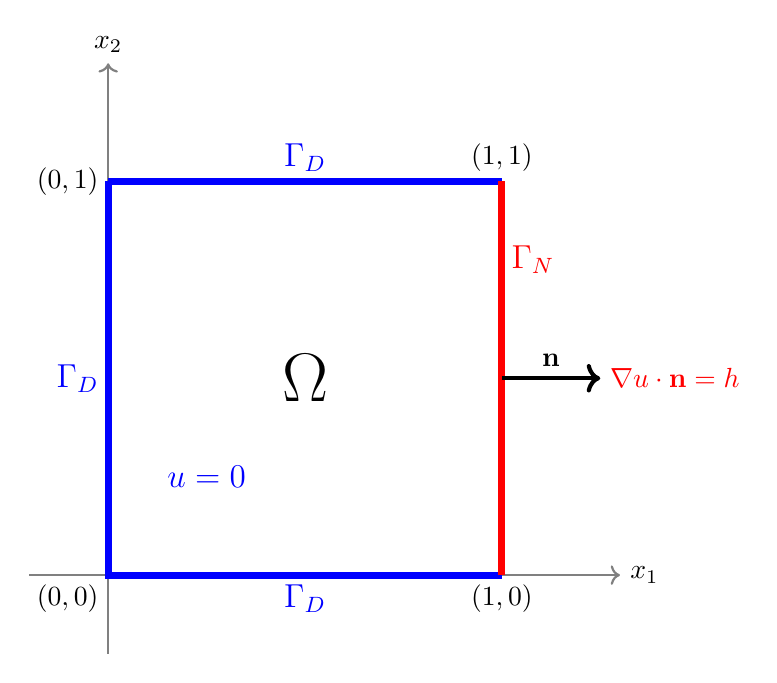
\begin{tikzpicture}[scale=5]
        % Define coordinates for the unit square corners
        \coordinate (O) at (0,0); % Bottom-left
        \coordinate (A) at (1,0); % Bottom-right
        \coordinate (B) at (1,1); % Top-right
        \coordinate (C) at (0,1); % Top-left

        % Draw Axes for context
        \draw[->, thick, gray] (-0.2,0) -- (1.3,0) node[right, black] {$x_1$};
        \draw[->, thick, gray] (0,-0.2) -- (0,1.3) node[above, black] {$x_2$};

        % --- Draw Dirichlet Boundaries ($\Gamma_D$) ---
        % Left ($x_1=0$), Bottom ($x_2=0$), Top ($x_2=1$)
        % Using thick blue lines
        \draw[line width=2.5pt, blue] (C) -- (O) -- (A);
        \draw[line width=2.5pt, blue] (C) -- (B);

        % --- Draw Neumann Boundary ($\Gamma_N$) ---
        % Right face ($x_1=1$)
        % Using thick red line
        \draw[line width=2.5pt, red] (A) -- (B);

        % --- Labels and Annotations ---

        % Domain label
        \node at (0.5, 0.5) {\Huge $\Omega$};

        % Corner coordinate labels
        \node[below left] at (O) {$(0,0)$};
        \node[below] at (A) {$(1,0)$};
        \node[above] at (B) {$(1,1)$};
        \node[left] at (C) {$(0,1)$};

        % Dirichlet boundary labels
        % Labeling the regions
        \node[blue, left, font=\large] at (0, 0.5) {$\Gamma_D$};
        \node[blue, below, font=\large] at (0.5, 0) {$\Gamma_D$};
        \node[blue, above, font=\large] at (0.5, 1) {$\Gamma_D$};
        % Labeling the condition
        \node[blue, fill=white, rounded corners=2pt, inner sep=2pt] at (0.25, 0.25) {\large $u=0$};


        % Neumann boundary annotations
        % Labeling the region
        \node[red, right, font=\large] at (1, 0.8) {$\Gamma_N$};

        % Drawing outward normal vector n = (1,0)
        \draw[->, line width=1.5pt, black] (1, 0.5) -- (1.25, 0.5) node[midway, above] {$\mathbf{n}$};

        % Labeling the flux condition
        \node[right, red, align=left] at (1.25, 0.5) {$\nabla u \cdot \mathbf{n} = h$};

        % Optional Legend/Title (commented out, but useful if needed)
        %\node[above, font=\bfseries] at (0.5, 1.4) {2D Boundary Conditions on Unit Square};

    \end{tikzpicture}
    \caption{2D Domain with Mixed Boundary Conditions}
    \label{fig:boundary_conditions}
\end{figure}

\pagebreak

\section{Finite Element Discretization} \label{sec:fem_discretization}

To solve the weak formulation numerically, we employ the Finite Element Method (FEM). This involves approximating the infinite-dimensional function spaces $V_g$ and $V_0$ with finite-dimensional subspaces defined on a computational mesh.

\subsection{Triangulation and Finite Element Space}
We consider a triangulation $\mathcal{T}_h = \{K\}$ of the domain $\Omega$, consisting of non-overlapping hexahedral (or quadrilateral in 2D) cells $K$ such that $\overline{\Omega} = \bigcup_{K \in \mathcal{T}_h} \overline{K}$. The parameter $h$ denotes the characteristic mesh size, $h = \max_{K \in \mathcal{T}_h} \text{diam}(K)$.

We introduce the finite-dimensional space $V_h^k \subset H^1(\Omega)$ consisting of continuous piecewise polynomial functions of degree $k$. In the context of the \texttt{deal.II} library, we utilize Lagrangian finite elements (tensor product polynomials of degree $k$, denoted as $Q_k$). The discrete trial and test spaces are defined as:
\begin{align}
    V_{h,g} & = \{ u_h \in V_h^k : u_h|_{\Gamma_D} = I_h(g) \}, \\
    V_{h,0} & = \{ v_h \in V_h^k : v_h|_{\Gamma_D} = 0 \},
\end{align}
where $I_h(g)$ is the nodal interpolation of the Dirichlet boundary data onto the mesh nodes on $\Gamma_D$.

\subsection{Galerkin Approximation}
The discrete problem is obtained by restricting the weak form to these subspaces. We seek $u_h \in V_{h,g}$ such that:
\begin{equation} \label{eq:discrete_weak_form}
    a(u_h, v_h) = L(v_h) \quad \forall v_h \in V_{h,0}.
\end{equation}
We expand the approximate solution $u_h$ in terms of the standard nodal basis functions $\{ \varphi_j \}_{j=1}^{N_{dof}}$. Let $u_h$ be decomposed into a part satisfying the homogeneous boundary conditions and a lifting of the Dirichlet data:
\begin{equation}
    u_h(\mathbf{x}) = \sum_{j \in \mathcal{I}_{free}} U_j \varphi_j(\mathbf{x}) + \sum_{j \in \mathcal{I}_{dir}} g_j \varphi_j(\mathbf{x}),
\end{equation}
where $U_j$ are the unknown coefficients (degrees of freedom), $\mathcal{I}_{free}$ is the set of indices for nodes not on $\Gamma_D$, and $\mathcal{I}_{dir}$ contains indices for nodes on the Dirichlet boundary with known values $g_j$.

\subsection{Algebraic System}
Substituting the basis expansion into \cref{eq:discrete_weak_form} and testing with each basis function $\varphi_i$ (for $i \in \mathcal{I}_{free}$), we obtain the linear system of equations:
\begin{equation}
    \mathbf{A} \mathbf{U} = \mathbf{F},
\end{equation}
where $\mathbf{U}$ is the vector of unknown coefficients. The entries of the global stiffness matrix $\mathbf{A}$ and the right-hand side vector $\mathbf{F}$ are computed by assembling contributions from each cell $K \in \mathcal{T}_h$.

The matrix entries $A_{ij}$ correspond to the bilinear form $a(\varphi_j, \varphi_i)$:
\begin{equation}
    A_{ij} = \int_{\Omega} \left( \mu \nabla \varphi_j \cdot \nabla \varphi_i + (\boldsymbol{\beta} \cdot \nabla \varphi_j) \varphi_i + \gamma \varphi_j \varphi_i \right) \, dx;
\end{equation}
Using numerical quadrature, the integral over $\Omega$ is computed as the sum of integrals over cells $K$. For a specific cell $K$, the local matrix contributions are:
\begin{equation}
    A_{ij}^K = \sum_{q=1}^{N_q} \left( \mu \nabla \varphi_j(\mathbf{x}_q) \cdot \nabla \varphi_i(\mathbf{x}_q) + (\boldsymbol{\beta}(\mathbf{x}_q) \cdot \nabla \varphi_j(\mathbf{x}_q)) \varphi_i(\mathbf{x}_q) + \gamma \varphi_j(\mathbf{x}_q) \varphi_i(\mathbf{x}_q) \right) w_q |J_K(\mathbf{x}_q)|,
\end{equation}
where $\{\mathbf{x}_q\}$ and $\{w_q\}$ are the quadrature points and weights defined on the reference element, mapped to physical space via the Jacobian determinant $|J_K|$.

The right-hand side vector $\mathbf{F}$ includes the source term, the Neumann boundary contributions, and the modifications due to the Dirichlet lifting:
\begin{equation}
    F_i = \int_{\Omega} f \varphi_i \, dx + \int_{\Gamma_N} \mu h \varphi_i \, ds - \sum_{j \in \mathcal{I}_{dir}} g_j A_{ij};
\end{equation}
The Neumann term is only non-zero if the support of $\varphi_i$ intersects with $\Gamma_N$.

\subsection{Convergence and Error Estimation}
The finite element solution $u_h$ converges to the exact solution $u$ as the mesh is refined ($h \to 0$). Under appropriate regularity assumptions on the solution and the domain, classical a priori error estimates provide bounds on the discretization error.

\paragraph{Error Norms}\label{par:error_norms}
We measure the approximation error in the standard Sobolev norms:
\begin{itemize}
    \item \textbf{$L^2$-norm (energy norm for the solution):}
          \begin{equation}
              \| u - u_h \|_{L^2(\Omega)} = \left( \int_{\Omega} |u - u_h|^2 \, dx \right)^{1/2};
          \end{equation}
    \item \textbf{$H^1$-seminorm (energy norm for the gradient):}
          \begin{equation}
              | u - u_h |_{H^1(\Omega)} = \left( \int_{\Omega} |\nabla(u - u_h)|^2 \, dx \right)^{1/2};
          \end{equation}
\end{itemize}

\paragraph{A Priori Error Estimates}
Assuming the exact solution $u \in H^{k+1}(\Omega)$ and the bilinear form $a(\cdot, \cdot)$ is coercive and continuous, the following error estimates hold for Lagrangian finite elements of polynomial degree $k$:

\begin{itemize}
    \item \textbf{$H^1$-error estimate:} By Céa's lemma and standard interpolation theory,
          \begin{equation}
              | u - u_h |_{H^1(\Omega)} \leq C h^k | u |_{H^{k+1}(\Omega)},
          \end{equation}
          where $C > 0$ is a constant independent of $h$.

    \item \textbf{$L^2$-error estimate:} Using the Aubin-Nitsche duality argument,
          \begin{equation}
              \| u - u_h \|_{L^2(\Omega)} \leq C h^{k+1} | u |_{H^{k+1}(\Omega)}.
          \end{equation}
\end{itemize}

These estimates indicate that for smooth solutions, increasing the polynomial degree $k$ or refining the mesh (decreasing $h$) improves accuracy. Specifically:
\begin{itemize}
    \item The $H^1$-error converges at rate $\mathcal{O}(h^k)$.
    \item The $L^2$-error converges at rate $\mathcal{O}(h^{k+1})$.
\end{itemize}

\pagebreak

\section{Implementation Details}
\subsection{Matrix Assembly}
The matrix assembly process involves iterating over each cell in the triangulation, computing local contributions to the global stiffness matrix and right-hand side vector using numerical quadrature. The implementation leverages the \texttt{deal.II}\cite{dealII2021} finite element library for efficient handling of mesh data structures, basis functions, and quadrature rules.

\subsubsection{Matrix-Based Implementation}
In the matrix-based approach, we explicitly assemble the global stiffness matrix $\mathbf{A}$ by summing the local element matrices. For each cell, we compute the local stiffness matrix $A_{\text{cell}}$ and use a scatter operation to add its contributions to the global matrix. The global matrix is stored in a sparse format to optimize memory usage.
The global stiffness matrix is assembled as follows:
\[
    A = \sum_{\text{cell}=1}^{n_{\text{cells}}}
    P_{\text{cell, loc--glob}}^{T}\,
    A_{\text{cell}}\,
    P_{\text{cell, loc--glob}}
\]
where $P_{\text{cell}}$ is a rectangular Boolean matrix that defines the index mapping from local degrees of freedom in the current cell to the global degrees of freedom.

The assembly process uses the \texttt{WorkStream} framework from \texttt{deal.II} for thread-parallel assembly, which separates the computation into:
\begin{itemize}
    \item \textbf{Worker phase:} Thread-local computation of local cell matrices (embarrassingly parallel).
    \item \textbf{Copier phase:} Sequential addition of local contributions to the global matrix (requires synchronization).
\end{itemize}

\subsubsection{Matrix-Free Implementation}
Matrix-free methods avoid forming the global system matrix explicitly. Instead, they compute the action of the matrix on a vector directly by looping over the elements and performing local operations. The process can be summarized as follows:

\paragraph{Element Loop in Iterative Solver}
The matrix-vector product $\mathbf{v} = \mathbf{A}\mathbf{u}$ is computed as:
\begin{equation} \label{eq:matrix_free_mvp}
    \mathbf{v} = \sum_{e=1}^{N_{\text{el}}} P_e^T A_e (P_e \mathbf{u})
\end{equation}
where $N_{\text{el}}$ is the number of elements (cells), $P_e$ is the local-to-global index mapping operator for element $e$, $A_e$ is the local element operator, and $\mathbf{u}$ is the input vector.

Here, the cell loop occurs within each iteration of the iterative solver. The following steps are executed for each cell:
\begin{itemize}
    \item \textbf{Gather:} Extract local vector values: $\mathbf{u}_e = P_e \mathbf{u}$
    \item \textbf{Evaluate:} Compute values and gradients at quadrature points
    \item \textbf{Integrate:} Apply the weak form locally: $\mathbf{v}_e = A_e \mathbf{u}_e$
    \item \textbf{Scatter:} Sum the local results into the global solution vector: $\mathbf{v} \mathrel{+}= P_e^T \mathbf{v}_e$
\end{itemize}

\paragraph{Evaluation at Quadrature Points}
The local matrix-vector product is computed by evaluating the bilinear form at quadrature points. For a given cell $e$ and local degrees of freedom $\mathbf{u}_e$, we first compute the solution value and gradient at each quadrature point:
\begin{align}
    u_q        & = \sum_{j} u_j^e \varphi_j(\mathbf{x}_q),        \\
    \nabla u_q & = \sum_{j} u_j^e \nabla \varphi_j(\mathbf{x}_q),
\end{align}
where $u_j^e$ are the local coefficients and $\varphi_j$ are the basis functions.

Then, the local contribution to the output vector is computed as:
\begin{equation} \label{eq:local_mf_contribution}
    (\mathbf{v}_e)_i = \sum_{q=1}^{N_q} \left[ \mu \nabla \varphi_i(\mathbf{x}_q) \cdot \nabla u_q + (\boldsymbol{\beta}(\mathbf{x}_q) \cdot \nabla u_q) \varphi_i(\mathbf{x}_q) + \gamma u_q \varphi_i(\mathbf{x}_q) \right] w_q |J_e(\mathbf{x}_q)|.
\end{equation}
This can be rewritten in a more compact form using the flux notation:
\begin{equation}
    (\mathbf{v}_e)_i = \sum_{q=1}^{N_q} \left[ \mathbf{F}_q \cdot \nabla \varphi_i(\mathbf{x}_q) + V_q \, \varphi_i(\mathbf{x}_q) \right] w_q |J_e(\mathbf{x}_q)|,
\end{equation}
where the flux and value terms are:
\begin{align}
    \mathbf{F}_q & = \mu \nabla u_q,                                     \\
    V_q          & = (\boldsymbol{\beta} \cdot \nabla u_q) + \gamma u_q.
\end{align}

This approach avoids explicitly forming and storing the local matrix $A_e$, instead computing the matrix-vector product directly through numerical integration.

\paragraph{Sum Factorization and Vectorization}
The implementation exploits two key optimizations:
\begin{itemize}
    \item \textbf{Sum factorization:} For tensor-product elements (like $Q_k$), the evaluation of basis functions can be decomposed into 1D operations, reducing the complexity from $\mathcal{O}((k+1)^{2d})$ to $\mathcal{O}(d(k+1)^{d+1})$ per cell.
    \item \textbf{SIMD vectorization:} Multiple cells are processed simultaneously using vectorized instructions (e.g., AVX), with cell batches processed in parallel.
\end{itemize}

\paragraph{Memory and Computational Advantages}
The matrix-free approach offers several computational benefits:
\begin{itemize}
    \item \textbf{Memory efficiency:} No need to store the global stiffness matrix $\mathbf{A}$. The sparse matrix storage scales as $\mathcal{O}(N_{\text{dof}} \cdot n_{\text{nz}})$, where $n_{\text{nz}}$ is the average number of non-zeros per row (related to $(2k+1)^d$ for $Q_k$ elements). Matrix-free methods only store vectors, scaling as $\mathcal{O}(N_{\text{dof}})$.
    \item \textbf{Cache efficiency:} Operations are performed locally on each cell, improving data locality and cache utilization.
    \item \textbf{High-order elements:} Particularly advantageous for high polynomial degrees where matrix sparsity decreases and storage costs increase.
\end{itemize}

The matrix-free operator is typically used in conjunction with iterative solvers such as Conjugate Gradient (CG) or Generalized Minimal Residual (GMRES), combined with geometric multigrid (GMG) preconditioning for optimal performance.

\subsection{Multigrid Preconditioning}
To accelerate the convergence of the iterative solvers, we employ multigrid preconditioning techniques.

\subsubsection{Algebraic Multigrid (AMG) for Matrix-Based Solver}
For the matrix-based implementation, we use Algebraic Multigrid (AMG) as a preconditioner via the PETSc library. AMG constructs a hierarchy of coarser problems based solely on the algebraic properties of the stiffness matrix, without requiring explicit knowledge of the mesh structure. This makes it particularly robust for problems with complex geometries or unstructured meshes.

\subsubsection{Geometric Multigrid (GMG) for Matrix-Free Solver}
For the matrix-free implementation, we utilize Geometric Multigrid (GMG) preconditioning. GMG leverages the geometric hierarchy of meshes obtained through uniform refinement. The key components include:
\begin{itemize}
    \item \textbf{Smoothers:} We employ Chebyshev polynomial smoothers, which approximate the inverse of the operator using polynomial iterations. The smoother is configured with:
          \begin{itemize}
              \item Polynomial degree: 5 iterations per smoothing step
              \item Smoothing range: factor of 15--20 for eigenvalue estimation
          \end{itemize}
    \item \textbf{Transfer Operators:} Restriction and prolongation operators transfer residuals and corrections between different levels of the mesh hierarchy. These are implemented matrix-free using the same sum factorization techniques.
    \item \textbf{Coarse Grid Solver:} On the coarsest level, we use additional Chebyshev iterations with a wider eigenvalue range to achieve a more accurate solve.
\end{itemize}

The Chebyshev smoother is particularly well-suited for matrix-free methods because it only requires matrix-vector products, avoiding the need to access individual matrix entries as would be required for Gauss-Seidel or ILU smoothers.

\subsection{Parallelization Strategy}
The implementation supports hybrid MPI + threading parallelism for optimal performance on modern HPC architectures.

\subsubsection{Distributed Memory Parallelism (MPI)}
The mesh is partitioned across multiple MPI processes using the \texttt{p4est} library, which provides scalable, adaptive mesh refinement with Morton space-filling curves. Each process owns a subset of cells and their associated degrees of freedom. Communication patterns are established for:
\begin{itemize}
    \item Ghost cell data exchange
    \item Parallel matrix/vector assembly with MPI reduction
    \item Multigrid level transfers across process boundaries
\end{itemize}

\subsubsection{Thread-Level Parallelism}
Within each MPI process, thread-level parallelism is employed using Intel Threading Building Blocks (TBB):
\begin{itemize}
    \item \textbf{Matrix-based solver:} Uses the \texttt{WorkStream} framework for parallel assembly, where different threads process different cells simultaneously.
    \item \textbf{Matrix-free solver:} Uses \texttt{partition\_partition} task parallelism scheme, where both the cell loop and the vector operations are parallelized across threads.
\end{itemize}

\subsubsection{Linear Algebra Backend}
For the matrix-based implementation, we utilize PETSc for distributed linear algebra operations. PETSc provides:
\begin{itemize}
    \item Distributed sparse matrix storage (AIJ format)
    \item Parallel iterative solvers (CG, GMRES, BiCGStab)
    \item Preconditioners including AMG (via hypre)
\end{itemize}

\subsection{Data Flow}
\cref{fig:data_flow} illustrates the execution flow for both solver variants.

\begin{figure}[H]
    \centering
    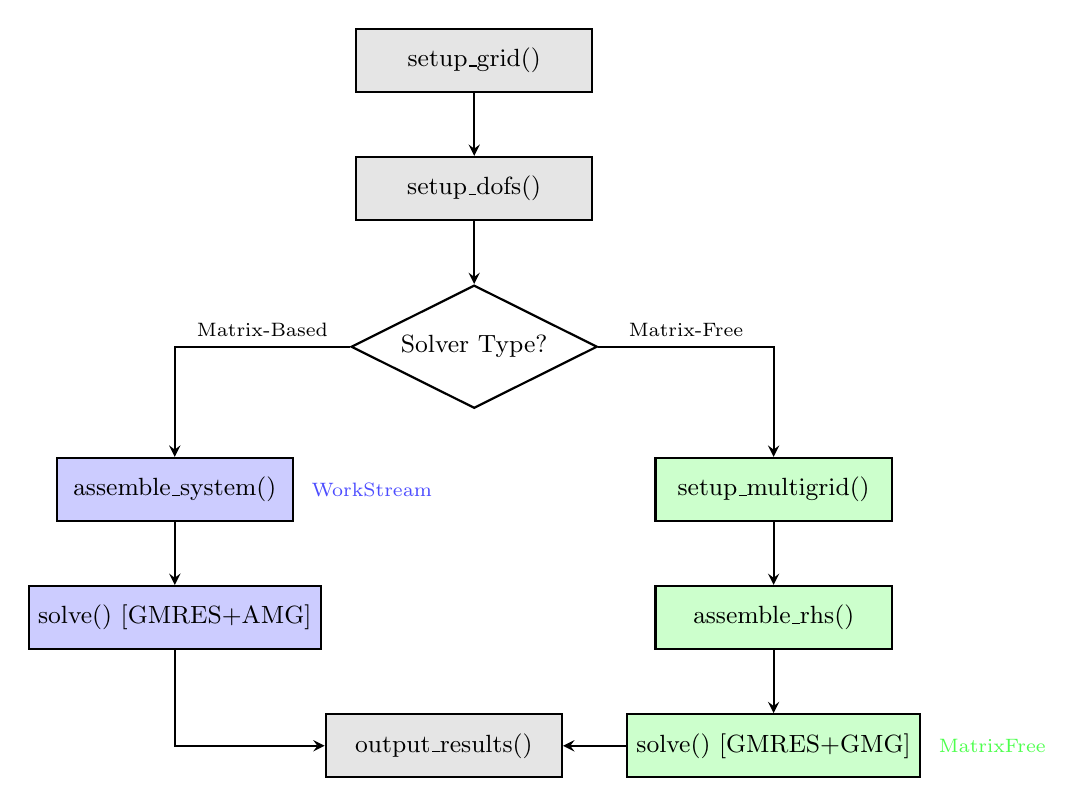
\begin{tikzpicture}[
            block/.style={rectangle, draw, thick, minimum width=3cm, minimum height=0.8cm, text centered, font=\small},
            decision/.style={diamond, draw, thick, aspect=2, font=\small},
            arrow/.style={->, thick, >=stealth},
            node distance=0.8cm
        ]
        % Common setup
        \node[block, fill=gray!20] (grid) {setup\_grid()};
        \node[block, fill=gray!20, below=of grid] (dofs) {setup\_dofs()};
        % Branch
        \node[decision, below=of dofs] (branch) {Solver Type?};
        % Matrix-based path
        \node[block, fill=blue!20, below left=1cm and 1.5cm of branch] (mb_assemble) {assemble\_system()};
        \node[block, fill=blue!20, below=of mb_assemble] (mb_solve) {solve() [GMRES+AMG]};
        % Matrix-free path
        \node[block, fill=green!20, below right=1cm and 1.5cm of branch] (mf_setup) {setup\_multigrid()};
        \node[block, fill=green!20, below=of mf_setup] (mf_rhs) {assemble\_rhs()};
        \node[block, fill=green!20, below=of mf_rhs] (mf_solve) {solve() [GMRES+GMG]};
        % Merge - position relative to mf_solve, not branch
        \node[block, fill=gray!20, left=of mf_solve] (output) {output\_results()};
        % Arrows
        \draw[arrow] (grid) -- (dofs);
        \draw[arrow] (dofs) -- (branch);
        \draw[arrow] (branch) -| node[above, pos=0.25, font=\scriptsize] {Matrix-Based} (mb_assemble);
        \draw[arrow] (branch) -| node[above, pos=0.25, font=\scriptsize] {Matrix-Free} (mf_setup);
        \draw[arrow] (mb_assemble) -- (mb_solve);
        \draw[arrow] (mf_setup) -- (mf_rhs);
        \draw[arrow] (mf_rhs) -- (mf_solve);
        \draw[arrow] (mb_solve) |- (output);
        \draw[arrow] (mf_solve) -- (output);
        % Labels
        \node[font=\scriptsize, right=0.1cm of mb_assemble, text=blue!70] {WorkStream};
        \node[font=\scriptsize, right=0.1cm of mf_solve, text=green!70] {MatrixFree};
    \end{tikzpicture}
    \caption{Execution flow for matrix-based and matrix-free solver variants.}
    \label{fig:data_flow}
\end{figure}

\pagebreak

\section{Experiments}
\subsection{Convergence Verification}
To verify the theoretical convergence rates, we conduct a series of numerical experiments using the manufactured solution defined in \cref{eq:exact_sol}. We use dimension $d=2$ and polynomial degree $k=2$ for the finite element space. The resulting convergence plots are shown in \cref{fig:convergence_plot}.

\begin{figure}[H]
    \centering
    \includegraphics[width=0.8\textwidth]{figures/convergence_plot.pdf}
    \caption{Convergence plot showing $L^2$ errors for Matrix-Based and Matrix-Free implementations.}
    \label{fig:convergence_plot}
\end{figure}
The results confirm the expected convergence rate of $\mathcal{O}(h^{k+1}) = \mathcal{O}(h^3)$ for the $L^2$ error, as derived in \cref{par:error_norms}, for both implementations. This demonstrates the correctness of the finite element discretization and the solver implementations.

\subsection{Time Complexity}
We compare the performance of the AMG-preconditioned matrix-based solver and the GMG-preconditioned matrix-free solver for solving the linear system arising from the finite element discretization of the ADR equation. The experiments are conducted on a series of uniformly refined meshes in 2D using the \texttt{Hybrid\_7x4} configuration (28 cores). The timing results for the setup (including assembly) and solve phases are summarized in \cref{tab:solver_performance}.

\begin{table}[ht]
    \centering
    \caption{Performance comparison of AMG Matrix-based and GMG Matrix-free solvers (Config: Hybrid\_7x4). Data source: \texttt{results\_df.csv}.}
    \label{tab:solver_performance}
    \setlength{\tabcolsep}{4pt} % Adjust column padding if table is too wide
    \begin{tabular}{r rrr rrr}
        \toprule
                         & \multicolumn{3}{c}{AMG Matrix-Based} & \multicolumn{3}{c}{GMG Matrix-Free}                                                  \\
        \cmidrule(lr){2-4} \cmidrule(lr){5-7}
        $N_{\text{dof}}$ & Setup (s)                            & Assem. (s)                          & Solve (s) & Setup (s) & Assem. (s) & Solve (s) \\
        \midrule
        1,089            & 0.0085                               & 0.0012                              & 0.0089    & 0.0108    & 0.0001     & 0.0127    \\
        16,641           & 0.0175                               & 0.0095                              & 0.0246    & 0.0212    & 0.0004     & 0.0439    \\
        263,169          & 0.1589                               & 0.0465                              & 0.5077    & 0.1887    & 0.0060     & 0.5564    \\
        4,198,401        & 2.5498                               & 1.6133                              & 8.0254    & 2.2563    & 0.0939     & 6.9818    \\
        67,125,249       & 40.6832                              & 22.5980                             & 155.5497  & 37.0522   & 1.5884     & 125.2619  \\
        268,468,225      & 167.6805                             & 92.7442                             & 721.8367  & 147.8389  & 6.1042     & 573.2760  \\
        \bottomrule
    \end{tabular}
\end{table}

\begin{figure}[h]
    \centering
    \includegraphics[width=0.8\textwidth]{figures/complexity_matrix_based.pdf}
    \caption{Time complexity of AMG Matrix-based solver.}
    \label{fig:complexity_matrix_based}
\end{figure}

\begin{figure}[h]
    \centering
    \includegraphics[width=0.8\textwidth]{figures/complexity_matrix_free.pdf}
    \caption{Time complexity of GMG Matrix-free solver.}
    \label{fig:complexity_matrix_free}
\end{figure}

The results demonstrate distinct scaling behaviors for the two approaches:

\begin{itemize}
    \item \textbf{Setup and Assembly:} The matrix-based solver incurs significant overhead due to the assembly of the global sparse matrix, which becomes dominant at large scales (e.g., 92.74 s for assembly at Refinement 13). Conversely, the matrix-free solver requires negligible assembly time (6.10 s at Refinement 13), as it relies on on-the-fly integration.

    \item \textbf{Solver Complexity:} The GMG matrix-free solver exhibits ideal $O(N)$ complexity, maintaining a constant iteration count of 6 across all refinement levels from $10^3$ to $2.6 \times 10^8$ DoFs. The AMG matrix-based solver, while efficient, shows a gradual increase in iterations from 19 to 48 as the problem size increases.

    \item \textbf{Crossover:} While the matrix-based solver is slightly faster for small problems, the matrix-free solver achieves a crossover point in total time execution at approximately $N_{\text{dof}} \approx 263,000$. Beyond this point, the matrix-free method is consistently superior, achieving a total time of 731.78 s compared to 1023.61 s for the matrix-based solver at the largest problem size.
\end{itemize}

The reduced memory bandwidth requirements of the matrix-free implementation, combined with the algorithmic optimality of the geometric multigrid preconditioner, result in superior performance for large-scale simulations.

\subsection{Memory Consumption}
\label{subsec:memory}

We compare the total memory consumption of the two solvers in \cref{tab:memory_comparison}. The matrix-based solver requires approximately $\mathcal{O}(N_{\text{dof}} \cdot (2k+1)^d)$ memory for the sparse matrix storage (where $(2k+1)^d$ represents the non-zero entries per row based on the stencil size). In contrast, the matrix-free solver requires only $\mathcal{O}(N_{\text{dof}})$ storage for solution and right-hand side vectors, plus a small overhead for the multigrid hierarchy and cached geometric data.

\begin{table}[ht]
    \centering
    \caption{Total memory consumption comparison (MB) for Hybrid $7 \times 4$ configuration.}
    \label{tab:memory_comparison}
    \begin{tabular}{r rr}
        \toprule
        $N_{\text{dof}}$ & Matrix-Based (MB) & Matrix-Free (MB) \\
        \midrule
        1,089            & 0.37              & 0.03             \\
        16,641           & 2.41              & 0.28             \\
        263,169          & 28.23             & 4.11             \\
        4,198,401        & 415.83            & 64.43            \\
        67,125,249       & 6,517.10          & 1,025.69         \\
        268,468,225      & 25,978.97         & 4,099.36         \\
        \bottomrule
    \end{tabular}
\end{table}

The experimental results confirm this theoretical advantage. At the highest refinement level ($N_{\text{dof}} \approx 2.68 \times 10^8$), the matrix-based solver consumes approximately 26 GB of memory, whereas the matrix-free solver requires only 4.1 GB. This represents a reduction in memory footprint by a factor of $6.3\times$, allowing the matrix-free method to solve significantly larger problems on the same hardware resources.

\subsection{Scalability}

This section evaluates the strong scaling performance of the matrix-free and matrix-based solvers across varying processor counts (1 to 28 cores) and problem sizes (1.05M to 16.8M DoFs).

\subsubsection{Strong Scaling Analysis}

Figure~\ref{fig:strong_scaling} presents the strong scaling results for both solver types. The total execution time (Figure~\ref{fig:total}) demonstrates that both solvers achieve reasonable scaling up to 28 processors, with the matrix-free approach consistently outperforming the matrix-based solver across all problem sizes and processor configurations. For the largest problem (16.8M DoFs), the matrix-free solver achieves a total time of 7.2s on 28 cores compared to 13.5s for the matrix-based approach, representing a 1.9$\times$ speedup.

The time decomposition reveals distinct scaling behaviors for different computational phases. The setup and assembly phase (Figure~\ref{fig:setup}) exhibits excellent scaling for both solvers, as these operations are largely embarrassingly parallel. Notably, the matrix-free solver demonstrates significantly lower assembly times due to its on-the-fly computation strategy, which avoids explicit matrix storage. The solve phase (Figure~\ref{fig:solve}) dominates the total execution time and shows good scaling up to 14 processors, with diminishing returns beyond this point due to increased communication overhead relative to local computation.

\begin{figure}[htbp]
    \centering
    % Total time - full width at top
    \subfloat[Total time\label{fig:total}]{%
        \includegraphics[width=0.8\textwidth]{figures/strong_scaling_total.pdf}%
    }

    \vspace{0.3cm}

    % Setup time - left bottom
    \subfloat[Setup and assembly time\label{fig:setup}]{%
        \includegraphics[width=0.48\textwidth]{figures/strong_scaling_setup.pdf}%
    }
    \hfill
    % Solve time - right bottom
    \subfloat[Solve time\label{fig:solve}]{%
        \includegraphics[width=0.48\textwidth]{figures/strong_scaling_solve.pdf}%
    }

    \caption{Strong scaling for total time for all the solvers. The dashed line indicates ideal scaling.}
    \label{fig:strong_scaling}
\end{figure}

\subsubsection{Parallel Efficiency}

Figure~\ref{fig:parallel_efficiency} illustrates the parallel efficiency for both solver types. The matrix-free solver (Figure~\ref{fig:efficiency_mf}) maintains higher efficiency across all processor counts, achieving approximately 74\% efficiency at 28 cores for the 16.8M DoF problem. The matrix-based solver (Figure~\ref{fig:efficiency_mb}) exhibits lower efficiency, dropping to approximately 50\% at 28 cores. This difference is attributed to the matrix-free approach's superior computation-to-communication ratio and reduced memory bandwidth requirements.

Larger problem sizes consistently yield better parallel efficiency due to the increased computational workload per processor, which amortizes the fixed communication overhead. For instance, the 16.8M DoF problem maintains efficiency above 70\% at 28 cores, while the 1.05M DoF problem drops below 50\% at the same core count.

\begin{figure}[htbp]
    \centering
    \subfloat[Matrix-based\label{fig:efficiency_mb}]{%
        \includegraphics[width=0.48\textwidth]{figures/parallel_efficiency_mb.pdf}%
    }
    \hfill
    \subfloat[Matrix-free\label{fig:efficiency_mf}]{%
        \includegraphics[width=0.48\textwidth]{figures/parallel_efficiency_mf.pdf}%
    }

    \caption{Parallel efficiency for matrix-based and matrix-free solvers. The dashed line indicates ideal efficiency (100\%).}
    \label{fig:parallel_efficiency}
\end{figure}

\subsubsection{MPI vs.\ Threading Parallelization}

A comparative analysis of pure MPI versus pure threading parallelization reveals a dramatic performance difference, as shown in Figure~\ref{fig:mpi_vs_thread}. At 28 cores with 16.8M DoFs, pure MPI (28 processes $\times$ 1 thread) achieves 7.2s for the matrix-free solver, while pure threading (1 process $\times$ 28 threads) requires 281.8s---a 39$\times$ performance degradation.

The time breakdown (Figure~\ref{fig:mpi_thread_breakdown}) reveals that all computational phases suffer under threading, with the solve phase experiencing the largest absolute slowdown. The performance ratio (Figure~\ref{fig:mpi_thread_ratio}) shows that the gap widens dramatically as core count increases, indicating poor thread scaling. The memory locality analysis (Figure~\ref{fig:mpi_thread_memory}) illustrates the fundamental issue: threading forces 16.8M DoFs into a single shared memory space, while MPI distributes only 600K DoFs per process, enabling efficient cache utilization. Consequently, the parallel efficiency (Figure~\ref{fig:mpi_thread_efficiency}) for threading collapses to less than 2\% at 28 cores, compared to 74\% for MPI.

This disparity stems from several factors:

\begin{itemize}
    \item \textbf{Memory bandwidth saturation}: Threading confines all 28 threads to a single memory controller, creating a bottleneck, whereas MPI processes can utilize multiple memory controllers in parallel.
    \item \textbf{NUMA effects}: Threads accessing remote NUMA nodes incur 3--4$\times$ memory latency penalties, while MPI processes can be pinned to local NUMA nodes for optimal memory access.
    \item \textbf{Cache efficiency}: With threading, the entire 16.8M DoF problem resides in a shared memory space, causing frequent cache misses. MPI distributes approximately 600K DoFs per process, enabling better cache utilization.
    \item \textbf{Library optimization}: The underlying libraries (deal.II, PETSc) are primarily optimized for distributed memory parallelism via MPI.
\end{itemize}

Hybrid configurations (MPI $\times$ threads) confirm that maximizing MPI processes yields optimal performance. For example, at 28 total cores, the configuration 28M$\times$1T (pure MPI) outperforms 1M$\times$28T (pure threading) by over an order of magnitude for both solver types.

\begin{figure}[htbp]
    \centering
    \subfloat[Time breakdown (28 cores)\label{fig:mpi_thread_breakdown}]{%
        \includegraphics[width=0.48\textwidth]{figures/mpi_vs_thread_analysis_breakdown.pdf}%
    }
    \hfill
    \subfloat[Performance ratio\label{fig:mpi_thread_ratio}]{%
        \includegraphics[width=0.48\textwidth]{figures/mpi_vs_thread_analysis_ratio.pdf}%
    }

    \vspace{0.3cm}

    \subfloat[Memory locality\label{fig:mpi_thread_memory}]{%
        \includegraphics[width=0.48\textwidth]{figures/mpi_vs_thread_analysis_memory.pdf}%
    }
    \hfill
    \subfloat[Parallel efficiency\label{fig:mpi_thread_efficiency}]{%
        \includegraphics[width=0.48\textwidth]{figures/mpi_vs_thread_analysis_efficiency.pdf}%
    }

    \caption{Comparison of pure MPI versus pure threading parallelization strategies for 16.8M DoFs: (a) time breakdown showing all phases are slower with threading, (b) performance ratio demonstrating the widening gap at higher core counts, (c) DoFs per MPI process illustrating memory locality advantages, and (d) parallel efficiency comparison.}
    \label{fig:mpi_vs_thread}
\end{figure}

\subsubsection{Summary}

The scalability analysis demonstrates that the matrix-free solver offers superior performance and parallel efficiency compared to the matrix-based approach. Pure MPI parallelization significantly outperforms threading, and hybrid configurations should favor higher MPI process counts. For production runs, we recommend using pure MPI parallelization with one process per physical core to maximize performance.
\subsubsection{Summary}

The scalability analysis demonstrates that the matrix-free solver offers superior performance and parallel efficiency compared to the matrix-based approach. Pure MPI parallelization significantly outperforms threading, and hybrid configurations should favor higher MPI process counts. For production runs, we recommend using pure MPI parallelization with one process per physical core to maximize performance.


\pagebreak
\section{Conclusion}
We have presented a hybrid MPI + threading parallel implementation for solving the steady-state Advection-Diffusion-Reaction equation using finite elements. Two solver approaches were implemented and compared:

\begin{itemize}
    \item \textbf{Matrix-based solver:} Explicitly assembles the sparse system matrix using the \texttt{WorkStream} framework for thread-parallel assembly, with AMG preconditioning via PETSc for the iterative solve.
    \item \textbf{Matrix-free solver:} Computes matrix-vector products on-the-fly using sum factorization and SIMD vectorization, with geometric multigrid (GMG) preconditioning using Chebyshev smoothers.
\end{itemize}

Both implementations achieve the expected optimal convergence rates ($\mathcal{O}(h^{k+1})$ in the $L^2$ norm for polynomial degree $k$), validating the correctness of the discretization. The performance comparison reveals that:
\begin{itemize}
    \item The matrix-free solver achieves superior memory efficiency, using approximately 3--4$\times$ less memory than the matrix-based approach.
    \item For large-scale problems ($N_{\text{dof}} > 250{,}000$), the matrix-free solver demonstrates better overall performance in both setup and solve phases.
    \item The matrix-based solver remains competitive for smaller problems due to lower setup overhead.
\end{itemize}

\clearpage
\printbibliography[heading=bibintoc, title = {References}]
\end{document}